\mysubsection{典型问题的描述}

之前已经提过,本章的核心问题是讨论函数列(族)的特定性质在取定极限之后是否能得到保持. 例如,一个重要的例子为:

\begin{itemize}
    \item 设 $f_n:\RR\to\RR$ 均连续,且 $f_n\to f:\RR\to\RR$. 问:$f$ 是否在 $\RR$ 上也连续?
\end{itemize}

其形式化的表述为

\begin{center}
    \begin{tikzcd}
        \lim\limits_{x\to x_0}f(x) \dar[equal,"?"] \rar[equal] & \lim\limits_{x\to x_0}\lim\limits_{n\to\infty}f_n(x) \drar[equal,"?",red] \\
        f(x_0) \rar[equal] & \lim\limits_{n\to\infty}f_n(x_0) \rar[equal] & \lim\limits_{n\to\infty}\lim\limits_{x\to x_0}f_n(x)
    \end{tikzcd}
\end{center}

从而 $f$ 是否连续的问题形式上表述为两个极限运算是否可以交换次序.

事实上,我们发现其它类似的问题最终也可以转化为这样一个抽象的交换极限次序的问题. 为此,我们首先来研究这个抽象的问题.

\mysubsection{两个极限可交换的充分条件}

\begin{theorem}\label{sl}
    设 $X,T$ 是两个集合. $\mathcal{B}_X,\mathcal{B}_T$ 分别是 $X,T$ 的一个基.

    设 $\set{f_t:X\to\RR|t\in T}$ 是一族函数. 若

    \begin{enumerate}
        \item\label{slcon1} $f_t\underset{\mathcal{B}_T}{\rightrightarrows}f:X\to\RR$.
        
        \item\label{slcon2} $\forall t\in T,\lim\limits_{\mathcal{B}_X}f_t(x)=A_t$
    \end{enumerate}

    则极限 $\lim\limits_{\mathcal{B}_T}A_t$ 与 $\lim\limits_{\mathcal{B}_X}f(x)$ 均存在且
$$
\lim_{\mathcal{B}_T}\lim_{\mathcal{B}_X}f_t(x)=\lim_{\mathcal{B}_T}A_t=\lim_{\mathcal{B}_X}f(x)=\lim_{\mathcal{B}_X}\lim_{\mathcal{B}_T}f_t(x)
$$
\end{theorem}

在证明这一结论之前,我们首先来理解一下定理的内容:

考虑以下的图表

\begin{center}
    \begin{adjustbox}{scale=1.5}
        \begin{tikzcd}[column sep={3cm,between origins},row sep={3cm,between origins}]
            f_t(x) \dar["\mathcal{B}_X"] \rar["\mathcal{B}_T",transform canvas={yshift=0.45ex}] \rar[transform canvas={yshift=-0.45ex}] & f(x) \dar["\mathcal{B}_X"]\\
            A_t \rar["\mathcal{B}_T"] & A
        \end{tikzcd}
    \end{adjustbox}
\end{center}

条件 \ref{slcon1} 对应上面的行,条件 \ref{slcon2} 对应左边的列.

定理假设左上半三角形之后得到的结论是:

下面的行成立,右面的列成立,且二者相等. 特别的,两条路线(右-下,下-右)得到同样的结论. 即上面的图表交换. 而这恰好说明两个极限可交换.

\begin{proof}
    \begin{enumerate}
        \item $\lim\limits_{\mathcal{B}_T}A_t$ 存在
        
        任取 $\eps>0$,由 $f_t\underset{\mathcal{B}_T}{\rightrightarrows}f$ 知
$$
\exists B_t\in\mathcal{B}_T,\forall t\in B_T,\forall x\in X,\abs{f_t(x)-f(x)}<\eps
$$

        任取 $t,t'\in B_T$. 由 $\lim\limits_{\mathcal{B}_X}f_t(x)=A_t,\lim\limits_{\mathcal{B}_X}f_{t'}(x)=A_{t'}$ 知
$$
\begin{aligned}
    &\exists B_X^1\in\mathcal{B}_X,\forall x\in B_X^1,\abs{f_t(x)-A_t}<\eps\\
    &\exists B_X^2\in\mathcal{B}_X,\forall x\in B_X^2,\abs{f_{t'}(x)-A_{t'}}<\eps
\end{aligned}
$$

        设 $B_X\in\mathcal{B}_X$ 满足 $B_X\subset B_X^1\cap B_X^2$. 从而对 $\forall x\in\mathcal{B}_X$ 有
$$
\abs{A_t-A_{t'}}\le\abs{A_t-f_t(x)}+\abs{f_t(x)-f(x)}+\abs{f(x)-f_{t'}(x)}+\abs{f_{t'}(x)-A_{t'}}<4\eps
$$

        从而 $\set{A_t}$ 确为 Cauchy 列.

        故存在唯一的 $A\in\RR$ 使得 $\lim\limits_{\mathcal{B}_T}A_t=A$.

        \item $\lim\limits_{\mathcal{B}_X}f(x)=A$
        
        任取 $\eps>0$. 设 $B_T$ 同前. 由 $\lim_{\mathcal{B}_T}A_t=A$ 知
$$
\exists B_T'\in\mathcal{B}_T,\forall t\in B_T',\abs{A_t-A}<\eps
$$

        任取 $t\in B_T\cap B_T'$. 则由 $\lim\limits_{\mathcal{B}_X}f_t(x)=A_t$ 知
$$
\exists B_X'\in\mathcal{B}_X,\forall x\in B_X',\abs{f_t(x)-A_t}<\eps
$$

        从而对 $\forall x\in B_X'$ 有
$$
\abs{f(x)-A}\le\abs{f(x)-f_t(x)}+\abs{f_t(x)-A_t}+\abs{A_t-A}<3\eps
$$

        即证 $\lim\limits_{\mathcal{B}_X}f(x)=A$.
    \end{enumerate}
\end{proof}

\begin{hint}
    \begin{enumerate}
        \item 从证明的过程可知,我们可以将到达域换成任何完备度量空间 $(Y,\rho)$.
        
        \item 若我们事先假设了 $\lim\limits_{\mathcal{B}_T}A_t$ 的存在性,则我们甚至不需要 $Y$ 完备.
    \end{enumerate}
\end{hint}

\mysubsection{极限与连续性}

作为第一个应用,我们来讨论极限函数的连续性.

\begin{theorem}
    设 $X$ 为度量空间,$f_t:X\to\RR,t\in T$ 是一族函数. 设 $\mathcal{B}$ 是 $T$ 的一个基.

    若以下两个条件成立:

    \begin{enumerate}
        \item $f_t\underset{\mathcal{B}}{\rightrightarrows}{f}$
        
        \item 对任意 $t\in T$ 均有 $f_t$ 在 $x_0\in X$ 处连续.
    \end{enumerate}

    则 $f$ 也在 $x_0$ 处连续.
\end{theorem}
\begin{proof}
    对 $X$ 的基 $x\to x_0$ 应用上一节的定理即得.
\end{proof}

\begin{inference}
    设 $X$ 为度量空间,$f_n:X\to\RR$ 均在 $X$ 上连续.

    若 $f_n\rightrightarrows f$,则 $f$ 也在 $X$ 上连续.
\end{inference}

\begin{inference}
    设 $X$ 为度量空间,$f_n:X\to\RR$ 均在 $X$ 上连续.

    若 $\sum\limits_{n=1}^\infty f_n(x)$ 在 $X$ 上一致收敛,则 $\sum\limits_{n=1}^\infty f_n(x)$ 也在 $X$ 上连续.
\end{inference}

现在我们可以强化第二节的一个性质:

\begin{property}[Abel]
    设幂级数 $\sum\limits_{n=0}^\infty a_n(z-z_0)^n$ 在 $z=\xi\ne z_0$ 处收敛.
    
    则 $\sum\limits_{n=0}^\infty a_n(z-z_0)^n$ 在区间 $[z_0,\xi]$ 上一致收敛,且该极限函数在 $[z_0,\xi]$ 上连续.
\end{property}
\begin{proof}
    我们已知级数在 $[z_0,\xi]$ 上一致收敛.

    又 $f_n(z)\triangleq a_n(z-z_0)^n$ 在 $[z_0,\xi]$ 上连续,则由上一推论知该级数在 $[z_0,\xi]$ 上也连续.
\end{proof}

\begin{example}[ Abel 求和]
    在历史上,人们经常需要考虑如何定义 $\sum\limits_{n=0}^\infty c_n$ 的值,以及如何求其具体值.

    情形 1:若已知 $\sum\limits_{n=0}^\infty c_n$ 收敛,则上述性质告诉我们:

    若定义 $\varphi(z)\triangleq\sum\limits_{n=0}^\infty c_nz^n$,则 $\varphi$ 在 $[0,1]$ 上连续. 从而
$$
\sum_{n=0}^\infty a_n=\lim_{z\to 1-}\varphi(z)=\varphi(1)
$$

    情形 2:有时甚至在 $\sum\limits_{n=0}^\infty c_n$ 不收敛的情形,如上定义的函数 $\varphi$ 仍在 $1$ 处有极限. 如
$$
\begin{aligned}
    \sum_{n=0}^\infty (-1)^n\longrightarrow \varphi(z)&=\sum_{n=0}^\infty (-1)^nz^n,\abs{z}<1\\
    &=\frac{1}{1+z}
\end{aligned}
$$

    从而 $\varphi(1)=\lim\limits_{z\to 1-}\varphi(z)=\dfrac{1}{2}$.

    故我们可以定义 $\sum\limits_{n=0}^\infty(-1)^n\triangleq\dfrac{1}{2}$.
\end{example}

\begin{example}
    设 $\alpha>0$ 且 $\alpha\notin\mathbb{N}$. 考虑级数
$$
\sum_{n=0}^\infty\frac{\alpha^{(n)}!}{n!}x^n=\sum_{n=0}^\infty\frac{\alpha(\alpha-1)\cdots(\alpha-n+1)}{n!}x^n
$$

    其可以由 $(1+x)^\alpha$ 作 Taylor 展开得到. 已知该级数的收敛半径为 $1$.
    
    从而对任意 $\abs{z}<1$ 有 $\sum\limits_{n=0}^\infty\dfrac{\alpha^{(n)}!}{n!}x^n$ 绝对收敛且 $\sum\limits_{n=0}^\infty\dfrac{\alpha^{(n)}!}{n!}x^n$ 在 $D_r$ 上一致收敛,其中 $0<r<1$.

    当 $x\in\RR$ 且 $\abs{x}<1$ 时,我们已知
$$
\sum_{n=0}^\infty\frac{\alpha^{(n)}!}{n!}x^n=(1+x)^\alpha
$$

    接下来我们来加强如上的结论.
\end{example}

\textbf{断言:}$\sum\limits_{n=0}^\infty\dfrac{\alpha^{(n)}!}{n!}$ 与 $\sum\limits_{n=0}^\infty\dfrac{\alpha^{(n)}!}{n!}(-1)^n$ 均收敛.

\begin{inference}
    $\sum\limits_{n=0}^\infty\dfrac{\alpha^{(n)}!}{n!}x^n$ 在区间 $[-1,1]$ 上一致收敛,且 $\sum\limits_{n=0}^\infty\dfrac{\alpha^{(n)}!}{n!}x^n=(1+x)^\alpha,x\in[-1,1]$.
\end{inference}
\begin{proof}
    由断言知,$\sum\limits_{n=0}^\infty\dfrac{\alpha^{(n)}!}{n!}x^n$ 在 $[-1,0]$ 与 $[0,1]$ 上均一致收敛,且连续.

    从而 $\sum\limits_{n=0}^\infty\dfrac{\alpha^{(n)}!}{n!}x^n$ 在 $[-1,1]$ 上一致收敛且连续.

    令 $\varphi(x)=\sum\limits_{n=0}^\infty\dfrac{\alpha^{(n)}!}{n!}x^n$. 已知 $\varphi(x)=(1+x)^\alpha,\abs{x}<1$.

    由二者均连续知
$$
\varphi(\pm 1)=\lim_{x\to\pm 1}\varphi(x)=\lim_{x\to\pm 1}(1+x)^\alpha=\begin{cases}
    2^\alpha & x=1\\
    0 & x=-1
\end{cases}
$$
\end{proof}

作为一个非常有趣的应用,我们有

\begin{inference}
    令 $\varphi(x)=\abs{x},x\in[-1,1]$. 则存在多项式列 $\set{P_n}$ 满足 $P_n(0)=0$ 且
$$
P_n\rightrightarrows\varphi,x\in[-1,1]
$$
\end{inference}
\begin{proof}
    我们已证 $\sum\limits_{n=0}^\infty\dfrac{\alpha^{(n)}!}{n!}y^n=(1+y)^\alpha,y\in[-1,1]$.

    令 $y=x^2-1,\alpha=\dfrac{1}{2}$. 其中 $x\in[-1,1]$. 则我们得到
$$
\sum\limits_{n=0}^\infty\dfrac{\left(\frac{1}{2}\right)^{(n)}!}{n!}(x^2-1)^n=\abs{x},x\in[-1,1]
$$

    由一致收敛性,定义
$$
\widetilde{P}_n(x)\triangleq\sum_{j=0}^n\frac{\left(\frac{1}{2}\right)^{(j)}!}{j!}(x^2-1)^j
$$

    则 $\widetilde{P}_n\rightrightarrows\abs{x},x\in[-1,1]$.

    取 $x=0$ 可得 $\widetilde{P}_n(0)\to 0$.

    令 $P_n(x)\triangleq\widetilde{P}_n(x)-\widetilde{P}_n(0)$.

    则 $P_n\rightrightarrows\abs{x},x\in[-1,1]$ 且 $P_n(0)=0$. 满足条件.
\end{proof}

以上我们从函数列的一致连续性得到极限函数的连续性.

接下来,我们讨论一个有趣的例子,我们从极限函数的连续性可以反推函数列的一致收敛.

\begin{property}[Dini]
    设 $K$ 为紧度量空间. 设 $f_n:K\to\RR$ 单调且连续.
    
    设 $f_n\to f:K\to\RR$ 连续. 则 $f_n\rightrightarrows f$.
\end{property}
\begin{proof}
    不妨设 $f_n$ 单调不升. 任取 $\eps>0$. 则
$$
\forall x\in K,\exists n_x\in\mathbb{N},f(x)\le f_{n_x}(x)<f(x)+\eps
$$

    由 $f_{n_x},f$ 均连续,存在 $x$ 的邻域 $U_x$ 使得
$$
\forall y\in U_x,f(y)\le f_{n_x}(y)<f(y)+\eps
$$

    则 $\set{U_x|x\in K}$ 为 $K$ 的开覆盖. 由 $K$ 紧,存在有限开覆盖 $\set{U_{x_1},\cdots,U_{x_m}}$.

    令 $N=\max\set{n_{x_1},\cdots,n_{x_m}}$.

    则对 $\forall n\ge N,\forall x\in K$ 存在 $i$ 使得 $x\in U_{x_i}$. 从而
$$
f(x)\le f_n(x)\le f_{n_i}(x)<f(x)+\eps
$$ 

    故 $f_n\rightrightarrows f$.
\end{proof}

\begin{inference}
    设 $K$ 为紧度量空间. 设 $f_n:K\to\RR_+$ 连续,且 $\sum\limits_{n=1}^\infty f_n(x)=f:K\to\RR_+$ 连续.

    则 $\sum\limits_{n=1}^\infty f_n(x)$ 在 $K$ 上一致收敛.
\end{inference}

\begin{example}
    设 $f_n:(0,\infty)\to\RR$ 为 $f_n(x)\triangleq n(1-x^\frac{1}{n})$.

    则 $\forall 0<a<b$ 在 $[a,b]$ 上有 $f_n\rightrightarrows\ln\frac{1}{x}$.

    但在 $(0,+\infty)$ 上 $f_n\not\rightrightarrows\ln\frac{1}{x}$.
\end{example}
\begin{proof}
    当 $x=1$ 时 $f_n(1)=0$.

    当 $x\ne 1$ 时,考虑函数 $\varphi(t)=x^t$. 则 $\varphi$ 为凸函数. 而
$$
f_n(x)=\frac{\varphi(0)-\varphi(\frac{1}{n})}{\frac{1}{n}}=-\frac{f(\frac{1}{n})-f(0)}{\frac{1}{n}-0}
$$

    为割线斜率的相反数.

    \begin{center}
        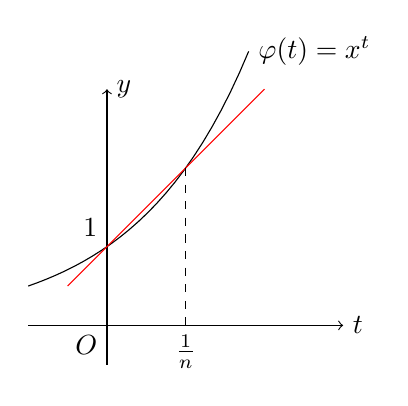
\begin{tikzpicture}
            \draw[->] (-1,0)--(3,0) node [right] {$t$};
            \draw[->] (0,-0.5)--(0,3) node [right] {$y$};
            \node at (0,0) [below left] {$O$};
            \node at (0,1) [above left] {$1$};
            \draw[domain=-1:1.8] plot(\x,{2^\x}) node [right] {$\varphi(t)=x^t$};
            \draw[-,red] (-0.5,0.5)--(2,3);
            \draw[-,dashed] (1,2)--(1,0) node [below] {$\frac{1}{n}$};
        \end{tikzpicture}
    \end{center}

    从而 $f_n(x)$ 单调不降且 $f_n(x)\to -\varphi'(0)=-\ln x=\ln\frac{1}{x}$.

    由 Dini 定理知在任何紧区间 $[a,b]\subset(0,\infty)$ 上有 $f_n\rightrightarrows\ln\frac{1}{x}$.

    但另一方面,若取定义域为 $(0,+\infty)$,则
$$
\Delta_n=\sup_{x\in(0,\infty)}\abs{f(x)-f_n(x)}=+\infty
$$

    从而 $\Delta_n\not\to 0$. 故 $f_n\not\rightrightarrows\ln\frac{1}{x}$.
\end{proof}

\mysubsection{极限与积分运算}

\begin{theorem}\label{ucint}
    设 $f_t:[a,b]\to\RR,t\in T$ 是一族函数. 设 $\mathcal{B}_T$ 是 $T$ 的一个基. 若

    \begin{enumerate}
        \item $f_t\underset{\mathcal{B}_T}{\rightrightarrows}f$
        
        \item $\forall t\in T,f_t\in\mathcal{R}[a,b]$
    \end{enumerate}

    则 $f\in\mathcal{R}[a,b]$ 且
$$
\int_a^bf(x)\dd x=\lim_{\mathcal{B}_T}\int_a^bf_t(x)\dd x
$$
\end{theorem}
\begin{proof}
    我们希望使用第 2 节的抽象定理 \ref{sl}. 为此,我们必须找到一个合适的框架:回忆积分是一种特殊的极限,其是关于一个特殊的空间的一个特殊的基取极限.

    定义 $X=\set{(P,\xi)|(P,\xi)\text{ 为 }[a,b]\text{ 带标志点的分划}}$.

    对任意 $\delta>0$ 令 $B_\delta=\set{(P,\xi)\in X|\lambda(P)<\delta}$.
    
    则 $\mathcal{B}_X=\set{B_\delta|\delta>0}$ 构成 $X$ 的一个基.

    考虑一族函数 $F_t:X\to\RR$ 定义为
$$
F_t(P,\xi)\triangleq\sigma(f_t,P,\xi)=\sum_{j=1}^nf_t(\xi_j)\Delta_j
$$

    由 $f_t\underset{\mathcal{B}_T}{\rightrightarrows}f$ 知 $F_t\underset{\mathcal{B}_T}{\rightrightarrows}F$. 其中 $F(P,\xi)\triangleq\sigma(f,P,\xi)$.

    由 $f_t\in\mathcal{R}[a,b]$ 知
$$
\lim_{\mathcal{B}_X}F_t(P,\xi)=\int_a^bf_t(x)\dd x=A_t
$$

    存在. 从而抽象定理的条件满足. 由该定理可得 $\lim\limits_{\mathcal{B}_T}A_t$ 与 $\lim\limits_{\mathcal{B}_X}F(P,\xi)$ 均存在且
$$
\lim_{\mathcal{B}_T}\int_a^bf_t(x)\dd x=\lim_{\mathcal{B}_T}A_t=\lim_{\mathcal{B}_X}F(P,\xi)=\int_a^bf(x)\dd x
$$
\end{proof}

\begin{inference}
    设 $f_n:[a,b]\to\RR$ 满足 $f_n\in\mathcal{R}[a,b]$.

    且 $\sum\limits_{n=1}^\infty f_n(x)$ 在 $[a,b]$ 上一致收敛,则 $\sum\limits_{n=1}^\infty f_n\in\mathcal{R}[a,b]$ 且
$$
\int_a^b\sum\limits_{n=1}^\infty f_n(x)\dd x=\sum_{n=1}^\infty\int_a^b f_n(x)\dd x
$$
\end{inference}

\begin{example}
    在第一卷我们定义过函数
$$
\mathrm{Si}(x)\triangleq\int_0^x\frac{\sin t}{t}\dd t
$$

    现在利用刚证的性质我们可以给出 $\mathrm{Si}(x)$ 的一个幂级数公式. 事实上
$$
\frac{\sin x}{x}=\sum_{n=0}^\infty\frac{(-1)^nx^{2n}}{(2n+1)!}
$$

    由其收敛半径为 $+\infty$ 知该幂级数在任何有界区间上均一致收敛. 从而由推论可知
$$
\begin{aligned}
    \mathrm{Si}(x)&=\int_0^x\frac{\sin t}{t}\dd t=\sum_{n=0}^\infty\frac{(-1)^n}{(2n+1)!}\int_0^xt^{2n}\dd t\\
    &=\sum_{n=0}^\infty\frac{(-1)^nx^{2n+1}}{(2n+1)!(2n+1)}
\end{aligned}
$$

    其收敛半径仍为 $+\infty$.

    特别的,在任何有界区间上,我们可以用多项式来一致逼近 $\mathrm{Si}(x)$.
\end{example}

\mysubsection{极限与微分运算}

接下来,我们讨论可微函数列在取完极限之后保持可微性的条件.

\begin{theorem}
    设 $X\subset\RR^n$ 为有界凸集. 设 $f_t:X\to\RR,t\in T$ 是一族函数. 设 $\mathcal{B}$ 是 $T$ 的一个基.

    若以下三个条件成立

    \begin{enumerate}
        \item $\forall t\in T,f_t$ 均在 $X$ 上可导.
        
        \item $f_t'\underset{\mathcal{B}}{\rightrightarrows}\varphi:X\to\RR$.
        
        \item $\exists x_0\in X,\lim\limits_{\mathcal{B}}f_t(x_0)$ 存在.
    \end{enumerate}

    则 $f_t\underset{\mathcal{B}}{\rightrightarrows}{f}$ 且 $f$ 在 $X$ 上可导,$f'=\varphi$.
\end{theorem}
\begin{proof}
    先证 $f_t\underset{\mathcal{B}}{\rightrightarrows}f$. 为此我们验证 Cauchy 准则:

    任取 $x\in X,t_1,t_2\in T$. 由有限增量定理
$$
\abs{f_{t_1}(x)-f_{t_2}(x)-(f_{t_1}(x_0)-f_{t_2}(x_0))}\le\sup_{\xi\in[x_0,x]}\abs{f_{t_1}'(\xi)-f_{t_2}'(\xi)}\abs{x-x_0}
$$

    由 $f_t'\underset{\mathcal{B}}{\rightrightarrows}\varphi$ 以及 $\lim\limits_{\mathcal{B}}f_t(x_0)$ 存在知
$$
\forall\eps>0,\exists B\in\mathcal{B},\forall t_1,t_2\in B,\forall x\in K,\abs{f_{t_1}'(x)-f_{t_2}'(x)}<\eps,\abs{f_{t_1}(x)-f_{t_2}(x)}<\eps
$$

    从而对 $\forall x\in X$ 有
$$
\abs{f_{t_1}(x)-f_{t_2}(x)}<\eps+\eps d(X)
$$

    由 Cauchy 准则知 $\set{f_t}$ 在 $\mathcal{B}$ 下一致收敛.

    记 $f_t\underset{\mathcal{B}}{\rightrightarrows}f$. 下证 $f$ 在 $X$ 上可微且 $f'=\varphi$.

    为此我们需证:若 $x\in X,x+h\in X$ 有
$$
F(h)\triangleq\frac{\abs{f(x+h)-f(x)-\varphi(x)h}}{\abs{h}}\to 0\quad(h\to 0)
$$

    我们希望使用定理 \ref{sl} 来证明该结论. 为此考虑
$$
F_t(h)\triangleq\frac{\abs{f_t(x+h)-f_t(x)-f_t'(x)h}}{\abs{h}}
$$

    一方面,对于固定的 $t\in T$ 由 $f_t$ 在 $x$ 处可导知
$$
\lim_{h\to 0}F_t(h)=0
$$

    另一方面,我们来验证 $F_t(h)\underset{\mathcal{B}}{\rightrightarrows}F(h)$.

    首先显然有 $F_t(h)\xrightarrow[\mathcal{B}]{}F(h)$.

    从而只需对 $\set{F_t(h):t\in T}$ 验证 Cauchy 准则.

    任取 $t_1,t_2\in T$ 由有限增量定理有
$$
\begin{aligned}
    &\abs{(f_{t_1}(x+h)-f_{t_1}(x)-f_{t_1}'(x)h)-(f_{t_2}(x+h)-f_{t_2}(x)-f_{t_2}'(x)h)}\\
    \le&\sup_{\xi\in[x,x+h]}\abs{(f_{t_1}'(\xi)-f_{t_2}'(\xi))-(f_{t_1}'(x)-f_{t_2}'(x))}\abs{h}
\end{aligned}
$$

    由 $f_t'\underset{\mathcal{B}}{\rightrightarrows}\varphi$ 知
$$
\forall\eps>0,\exists B\in\mathcal{B},\forall t_1,t_2\in B,\forall x\in X,\abs{f_{t_1}'(x)-f_{t_2}'(x)}<\eps
$$

    从而对 $\forall h\ne 0$ 有
$$
\abs{F_{t_1}(h)-F_{t_2}(h)}<\frac{(\eps+\eps)\abs{h}}{\abs{h}}=2\eps
$$

    即 $\set{F_t}$ 在 $\mathcal{B}$ 下一致收敛. 从而 $F_t\underset{\mathcal{B}}{\rightrightarrows}F$.

    现在由定理 \ref{sl} 知 $\lim\limits_{h\to 0}F(h)$ 与 $\lim\limits_{\mathcal{B}}\lim\limits_{h\to 0}F_t(h)$ 均存在且二者相等.

    从而 $\lim\limits_{h\to 0}F(h)=0$. 即 $f$ 在 $x$ 处可导且 $f'(x)=\varphi(x)$.
\end{proof}

\begin{inference}
    设 $X\subset\RR^n$ 为有界凸集. 设 $f_n:X\to\RR$ 在 $X$ 上可微.

    设 $\sum\limits_{n=1}^\infty f_n'(x)$ 在 $X$ 上一致收敛,且 $\exists x_0\in X,\sum\limits_{n=1}^\infty f_n(x_0)$ 收敛.

    则 $\sum\limits_{n=1}^\infty f_n(x)$ 在 $X$ 上一致收敛,极限函数可微且满足
$$
\left(\sum\limits_{n=1}^\infty f_n(x)\right)'=\sum\limits_{n=1}^\infty f_n'(x)
$$
\end{inference}

作为应用,我们来讨论幂级数的逐项求导与逐项积分.

\begin{property}
    设幂级数 $\sum\limits_{n=0}^\infty a_n(z-z_0)^n$ 的收敛半径 $R>0$. 则

    \begin{enumerate}
        \item 该幂级数在 $z_0+D_R$ 上 $C^{(1)}$ 光滑,且极限函数 $S$ 可微,有
$$
S'(x)=\sum_{n=1}^\infty na_n(z-z_0)^{n-1}
$$

        \item 对任意光滑路径 $\gamma:[0,1]\to z_0+D_r$ 满足 $\gamma(0)=z_0,\gamma(1)=z$ 有
$$
\int_\gamma S(z)\dd z=\sum_{n=0}^\infty\frac{a_n}{n+1}(z-z_0)^{n+1}
$$
    \end{enumerate}
\end{property}

\img{0.4}{16.3.1.png}

\begin{proof}
    \begin{enumerate}
        \item 在第一学期我们就证明过这个结论. 但在这里,我们用新的知识来重新证明一遍.
        
        令 $f_n(z)=a_n(z-z_0)^n$. 则 $f_n$ 可微且 $f_n'(z)=na_n(z-z_0)^{n-1}$.

        由 $\overline{\lim\limits_{n\to\infty}}\sqrt[n]{n\abs{a_n}}=\dfrac{1}{R}$ 知 $\sum\limits_{n=0}^\infty f_n'(z)$ 在 $z_0+D_r$ 上一致收敛,$\forall 0<r<R$.

        且 $\sum\limits_{n=0}^\infty f_n(z_0)$ 显然收敛. 从而由上一推论可知:$\sum\limits_{n=0}^\infty f_n(z)$ 也一致收敛且可微,且有
$$
\left(\sum_{n=0}^\infty a_n(z-z_0)^n\right)'=\sum_{n=1}^\infty na_n(z-z_0)^{n-1}
$$

        \item 取 $0<r<R$ 使得 $\gamma([0,1])\subset z_0+\overline{D_r}$.
        
        则由 $\sum\limits_{n=0}^\infty a_n(z-z_0)^n$ 在 $z_0+\overline{D_r}$ 上一致收敛知
$$
\sum\limits_{n=0}^\infty a_n(\gamma(t)-z_0)^n\gamma'(t)
$$

        在 $[0,1]$ 上一致收敛. 从而由积分与求和可交换次序知
$$
\begin{aligned}
    &\int_\gamma\sum\limits_{n=0}^\infty a_n(z-z_0)^n\dd z=\int_0^1\sum\limits_{n=0}^\infty a_n(\gamma(t)-z_0)^n\gamma'(t)\dd t\\
    =&\sum\limits_{n=0}^\infty a_n\int_0^1(\gamma(t)-z_0)^n\gamma'(t)\dd t=\sum_{n=0}^\infty a_n\int_0^1\frac{\dd(\gamma(t)-z_0)^{n+1}}{n+1}\\
    =&\sum\limits_{n=0}^\infty \frac{a_n}{n+1}(z-z_0)^{n+1}
\end{aligned}
$$
    \end{enumerate}
\end{proof}

\begin{example}
    Bessel 函数 $J_n(x)$ 为如下微分方程的解:
$$
x^2y''+xy'+(x^2-n^2)y=0
$$

    我们可以使用幂级数法来求解该方程.

    例如在 $n=0$ 时
$$
J_0(x)=1+\sum\limits_{k=1}^\infty(-1)^k\frac{x^{2k}}{(k!)^22^{2k}}
$$
\end{example}